\documentclass{../ficheTDTP}
\usepackage{hyperref}
\usepackage{tikz}
\usetikzlibrary{positioning,shapes,shadows,arrows,fit}

%\usepackage[utf8]{inputenc}
%\usepackage[french]{babel}
%\usepackage[T1]{fontenc}
%
%\usepackage[left=3cm, right=3cm, top=3cm, bottom=3cm]{geometry}
%\usepackage{amsmath}
%\usepackage{amsfonts}
%\usepackage{amssymb}
%%\usepackage{graphics}
%\usepackage{graphicx}
%\usepackage{listings}
%\usepackage{color}
%\usepackage{float}
%
%\newtheorem{de}{Définition}[section] % les définitions et les théorèmes sont
%\newtheorem{theo}{Théorème}[section]    % numérotés par section
%\newtheorem{prop}[theo]{Proposition}

\title{Projet Planètes}
\def \pname{planetes}


\begin{document}

\maketitle

\begin{figure}[h]
\vspace{-5mm}
	\begin{center}
            \includegraphics[width=8cm]{planetes.png}
        \end{center}
	
\end{figure}

\section*{Introduction}

Le but de ce projet est de modéliser un système planétaire. La modélisation de tels systèmes permet, par exemple, de prédire des événements astronomiques comme des éclipses, des \textit{conjonctions} (alignement de deux planètes vu d'une troisième), ou encore le passage d'une comète ou d'un astéroïde.

\textbf{Mots clés : simulation, géométrie, trigonométrie.}

Le principe du projet est d'étudier une question mathématique complexe de façon autonome et originale en utilisant l'outil informatique. \textbf{L'ensemble du projet est à faire par groupe de 3 étudiants.} Le projet est divisé en 2 sections : théorique et pratique. La première partie est \textbf{obligatoire}, la seconde partie correspond à des \textbf{pistes de travail}.

\subsection*{Rendu du projet}\strut

Vous devrez rendre:

\begin{itemize}

\item un \textbf{rapport de mi-projet} répondant aux questions de la section 1;

\item un \textbf{exposé} en fin de projet présentant votre travail et vos résultats sur la section 2.
\end{itemize}

\subsection*{Le rapport}\strut

\smallskip
\textbf{Date de rendu} : cf site du cours \url{https://www.lri.fr/~pons/teaching-mathinfo-l1.html}

\smallskip
\textbf{Que faut-il faire ?} Répondre aux questions de la section 1.

\smallskip
\textbf{Quel format ?} Format PDF obligatoire. Si vous souhaitez ajouter des dessins, vous pouvez les scanner et les ajouter à votre document.

\smallskip
\textbf{Qui réalise le rapport ?} Les membres du groupe réfléchissent ensemble au rapport mais rédigent chacun leur propre rapport. N'oubliez pas de préciser sur votre document qui sont les autres membres du groupe !

\smallskip
\textbf{Comment le rendre ?} Dans votre projet SageMathCloud, vous trouverez un dossier \og Rapport\fg, c'est là qu'il faut uploader votre rapport PDF.

\subsection*{L'exposé}\strut

\smallskip
\textbf{Quand ?} Les exposés auront lieu courant mai, la date sera précisée ultérieurement.

\smallskip
\textbf{Que doit-on présenter ?} Vous devez présenter le travail effecuté sur la section 2 du projet, en particulier les résultats que vous avez obtenus, les algorithmes que vous avez utilisés, les images ou vidéos produites, etc.

\smallskip
\textbf{En combien de temps ?} Vous aurez 10 minutes de présentation, puis 5 minutes de questions.

\smallskip
\textbf{Sur quel support ?} Vous aurez un vidéo projecteur et un ordinateur à disposition (ou le votre si vous le souhaitez). Vous pourrez donc présenter votre exposé sous forme d'un powerpoint ou pdf. Vous pouvez aussi montrer des images, vidéos, démos de code.

\smallskip
\textbf{Qui parle ?} Tout le monde ! Les 3 étudiants doivent participer.

\smallskip
\textbf{Doit-on présenter notre code ?} Vous pouvez utiliser un notebook SageMathCloud pour présenter des démos de code, cependant nous ne notons pas la programmation mais bien les résultats obtenus !

\smallskip
\textbf{Doit-on répondre aux questions ?} Les question de la section 2 ne sont pas obligatoires, ce sont des pistes de travail, vous pouvez les suivre, ou pas...


\section{Partie théorique}

\subsection{Un premier modèle (très) simplifié à $2$ planètes}$\;$\\

	Comme premier cas modèle, nous allons imaginer la situation de deux planètes $P_1$ et $P_2$ gravitant autour d'une étoile E (l'équivalent de notre Soleil). Le mouvement des planètes sera considéré \textbf{circulaire} autour de l'étoile E (voir figure \ref{fig1}) et on supposera qu'elles gravitent sur le même plan (voir plan \textit{écliptique}).
	
\begin{figure}[h]
	\begin{center}
            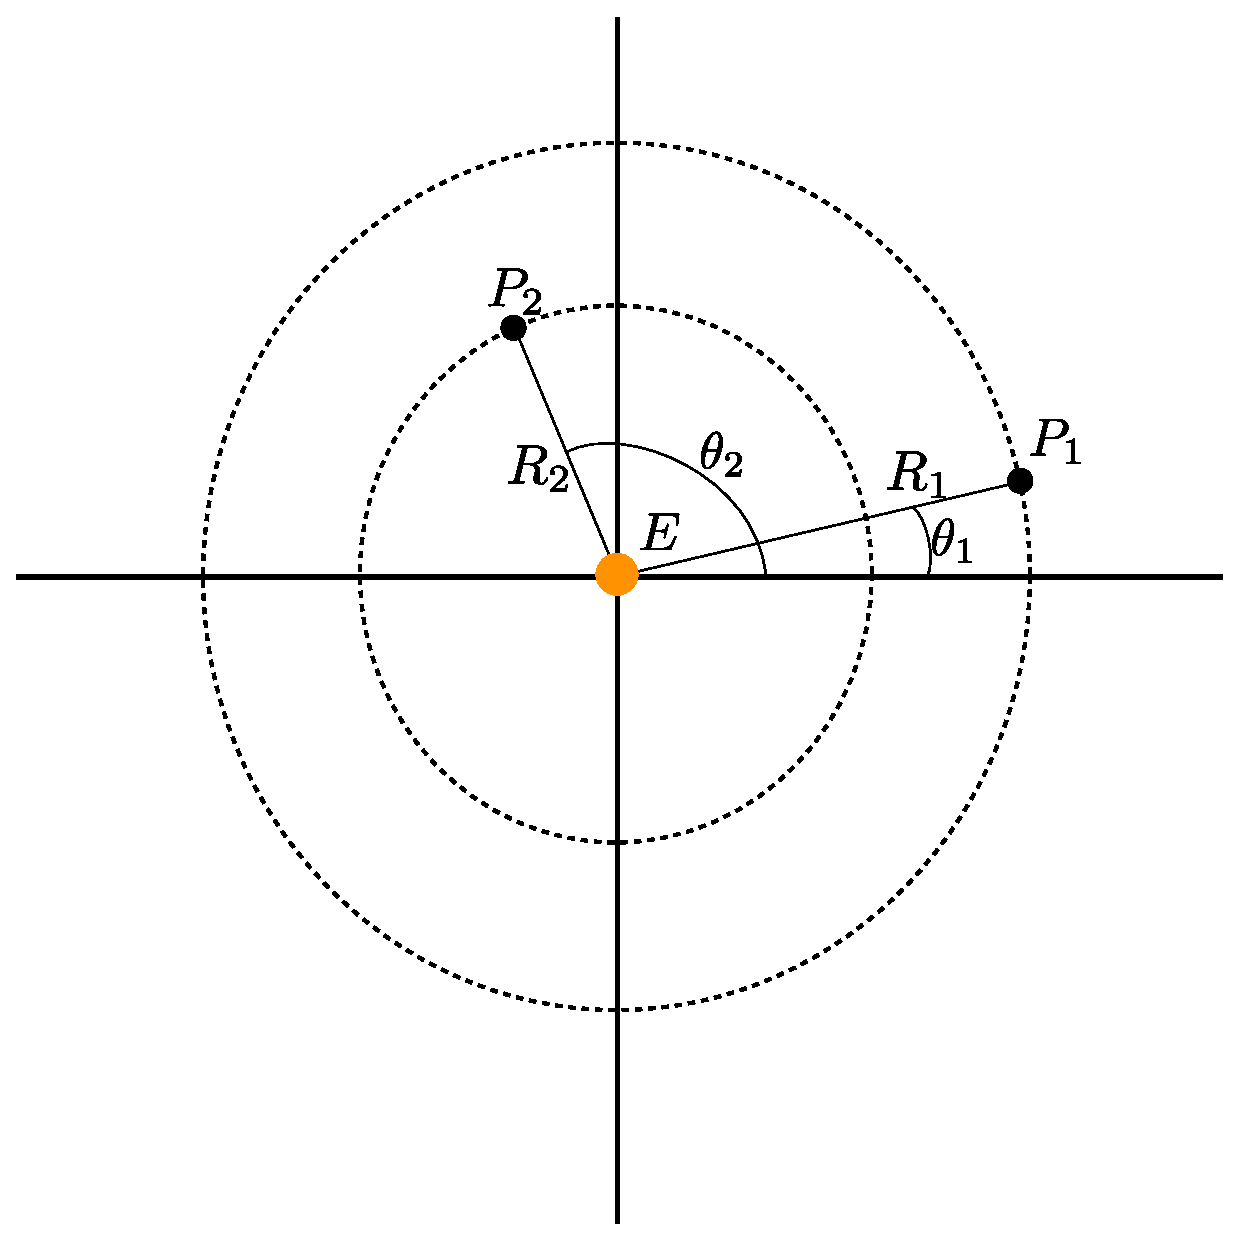
\includegraphics[width=6cm]{planete.eps}
        \end{center}
	\vspace{-5mm}
	\caption{Schéma représentatif du système à deux planètes $P_1$ et $P_2$ et notations.}\label{fig1}
\end{figure}	
	
	Afin de mettre en équations le mouvement des planètes, nous avons besoin de définir un repère. On considérera que E est le centre d'un repère orthonormé. Dans ce repère, les équations de mouvement des planètes seront simplement :
\[
	P_1 = R_1 (cos(\theta_1),sin(\theta_1)) \quad \text{et} \quad P_2 = R_2 (cos(\theta_2),sin(\theta_2)),
\]	
où $R_1>0$ et $R_2>0$ sont les rayons respectifs des trajectoires des planètes, et $\theta_1$ et $\theta_2$ les angles respectifs par rapport au repère.

 On notera dans la suite par $t$ le temps. On supposera que le mouvement des planètes obéit à la $2$ème \textbf{loi de Kepler}.

\subsection{Questions}

\begin{enumerate}

\item Donner l'évolution dans le temps du rayon $R_i$ ($i = \{1,2 \}$) et de l'angle $\theta_i$ de la planète $P_i$. On rappelle que les trajectoires sont \textit{parfaitement circulaires}, et qu'elles obéissent à la $2$ème loi de Kepler. Pour la suite, on notera par $v_1$ et $v_2$ les vitesses angulaires des deux planètes.

\item La planète Terre se situe à (environ) $150$ millions de kilomètres du Soleil. En considérant notre orbite parfaitement circulaire, donner la vitesse à laquelle on tourne autour de notre étoie (en km/s).\\

\noindent Étant donné un point d'observation $O$ situé en $(x_0,y_0)$ dans l'espace, il est possible de voir à certain moment un alignement des planètes.
	
\item En pla\c cant l'observateur $O$ au centre du repère (c'est à dire à la position $(x_0,y_0) = (0,0)$), donner une équation simple correspondant à l'alignement des planètes. En déduire (en fonction des vitesses $v_1$ et $v_2$) tous les temps $t$ pour lesquels les planètes $P_1$ et $P_2$ sont alignés.

\item Dépla\c cons maintenant notre observateur $O$ en $(x_0,y_0)$ fixé. De ce nouveau point de vu, donner une équation correspondant à l'alignement de $O$, $P_1$ et $P_2$. Généraliser au cas où $(x_0,y_0)$ n'est pas fixé (par exemple si l'observateur tourne autour de l'étoile).

\textbf{Indication} : $P_1 O$ et $P_2 O$ sont alignés ssi un vecteur (non nul) orthogonale à $P_1O$ (ou $P_2O$) est orthogonale à $P_2O$ (ou $P_1O$).\\


\noindent \textbf{Mouvement apparent des planètes : } Lorsqu'on observe le mouvement des planètes à partir du Soleil, il est clair que les planètes ont un mouvement circulaire (ou presque) autour de l'étoile. Cependant, sur terre, nous avons observé le mouvement des planètes à partir d'un astre en mouvement. La \textit{trajectoire apparente} des autres planètes n'est alors plus un cercle. Ce point avait notamment amené au modèle géocentrique pour décrire l'univers.\\

\item Donner l'équation de mouvement de l'étoile $E$ pour un observateur situé sur la planète $P_1$ (cela revient à un changement de repère centré en $P_1$).

\item De même donner l'équation du mouvement apparent de $P_2$ vu à partir de $P_1$. La courbe obtenue est-elle un cercle ? (la tracer) Justifier le modèle géocentrique autrefois proposé (voir \textit{epicycle}).\\

\noindent \textbf{Les éclipses : } Ajoutons à notre système à deux planètes un \textit{satellite} $S$ à la planète $P_1$. Une éclipse se produit sur la planète $P_1$ lorsque $S$ est aligné avec l'étoile $E$ et la planète $P_1$ et de plus que $S$ est situé entre les deux.\\

\item Donner l'équation du mouvement apparent du satellite $S$ vu de la planète $P_2$.

\item En supposant la trajectoire de $S$ parfaitement circulaire autour de $P_1$, donner une équation mathématique formalisant une éclipse. En déduire tous les temps $t$ pour lesquels cet événement se produit.

\item En comparant avec notre situation, que pensez vous du résultat de la question précédente (y a t'il autant d'éclipse sur Terre) ? Quelle hypothèse dans notre modèle provoque cette erreur ?

\end{enumerate}



	\section{Modélisation et extensions}
	
	Le but de cette partie sera d'explorer différentes extensions possibles de notre modèle et d'utiliser le logiciel sage pour visualiser notre résultats. Nous proposons ici quelques pistes d'études que vous pouvez compléter avec de nouvelles si vous le souhaitez.
	

	\subsection{Notre système solaire} Nous allons chercher à concevoir une animation permettant de visualiser au cours du temps le mouvement des planètes de notre système solaire.
	
\begin{enumerate}
	\item Commencer par représenter dans un graphique la trajectoire des $9$ (ou $8$) planètes de notre système solaire (pour l'instant sans animation). Trouver les distances entre les planètes (en Unité Astronomique) pour représenter à la bonne échelle.
	\item Ajouter sur ces trajectoires la position des planètes (par exemple par un disque) à un instant $t$. Essayer de récupérer sur internet la position relative des planètes à un instant donné.
	\item Animer votre simulation en faisant bouger les planètes au cours du temps (attention, il est nécessaire de connaître leurs vitesses).
	\item Ajouter à ce système les satellites de plusieurs planètes.
	\item Modifier votre code pour prendre en considération le mouvement elliptique des planètes. Essayer de prédire à l'aide de votre simulateur des conjonctions entre les différentes planètes du système solaire.
\end{enumerate}

	\subsection{Le système géocentrique} Revenons quelques (beaucoup) de siècles en arrière, et considérons que la Terre est le centre de notre système.
\begin{enumerate}
	\item En utilisant le système des épicycles, tracer dans un graphe $2$D la trajectoire des planètes vus de la Terre (ainsi que celle du soleil) (sans animation).
	\item En choisissant une position initial arbitraire pour les différentes planètes, faites une animation simulant le mouvement des planètes et du soleil vus de la Terre.
	\item Le modèle des épicycles possèdent certaines lacunes par rapport aux observations qu'on peut faire de la Terre. Essayer de simuler le système des \textit{épicycles excentrés}.
	\item Essayer d'enrichir votre simulateur avec le système de l'\textit{équant} introduit par Ptolémée.
\end{enumerate}


	\subsection{Envoie d'une sonde sur Mars} Essayer d'enrichir votre simulateur pour simuler l'envoi d'une sonde de la Terre vers Mars. 
	
\vspace{2cm}
\footnotesize{Image : Solar System, \url{https://commons.wikimedia.org/wiki/File:Solar_System_size_to_scale_fr.svg}}


	
\end{document}